\documentclass{article}
\usepackage{graphicx} % Required for inserting images
\usepackage{float}
\usepackage{media9}
\usepackage{xcolor}
\usepackage{amsmath}
% \usepackage{amsfonts}
\usepackage{geometry}[0.05in]
\usepackage{hyperref}
\usepackage{mathtools}
\usepackage[justification=centering]{caption}
\usepackage[most]{tcolorbox}
\usepackage{comment}
\usepackage{tikz}
\usepackage{parskip}
\usepackage[activate={true,nocompatibility},final,tracking=true,kerning=true,spacing=true,factor=1100,stretch=10,shrink=10]{microtype}
% fonts
\usepackage[p,osf]{cochineal}
\usepackage[scale=.95,type1]{cabin}
\usepackage[cochineal,bigdelims,cmintegrals,vvarbb]{newtxmath}
\usepackage[zerostyle=c,scaled=.94]{newtxtt}
\usepackage[cal=boondoxo]{mathalfa}

\newcommand{\todo}[1]{\textbf{\textcolor{red}{TODO: #1}}}
\newtcolorbox{questionbox}{enhanced,colback=blue!5!white,colframe=blue!10,boxrule=0.5pt,parbox=false}

\usepackage{soul}
\definecolor{Light}{rgb}{1, 0.9, 0.9}
\sethlcolor{Light}
\newcommand{\hltexttt}[1]{\texttt{\hl{#1}}}
\usetikzlibrary{decorations.text}

% Define colors (adjust the RGB values to your liking)
\definecolor{neuripscolor}{rgb}{0,0,0}

% argmin, argmax
\DeclareMathOperator*{\argmin}{argmin}
\DeclareMathOperator*{\argmax}{argmax}

\begin{document}
% Title Box
\noindent\colorbox{neuripscolor}{
    \parbox{\textwidth}{
        \color{white}
        \vspace{0.5cm}
        \centering
        \LARGE\textbf{Interactive Intelligence (I2) Grimoire}
        \vspace{0.5cm}
    }
}

\vspace{1cm}

\begin{center}
  {{UNIT}} UNIT
\end{center}

\vspace{1cm} % Space between title and text

\begin{tikzpicture}[every node/.style={align=center}]
    \centering
    % Settings
    \newcommand\NumOfAuthors{6}
    \newcommand\Radius{7cm} % Radius where the names are placed
    \newcommand\InnerRadius{3cm} % Radius for the inner connecting lines
    \newcommand\ImageRadius{1.5cm} % Radius of the central image area
    
    % Circle for authors
    \draw[line width=2pt, black] (0,0) circle (\ImageRadius + \InnerRadius);
    
    % Inner circle for connecting lines
    \draw[line width=1.5pt, gray, opacity=0.5] (0,0) circle (\InnerRadius);
    
    % Image in the center
    \node at (0,0) {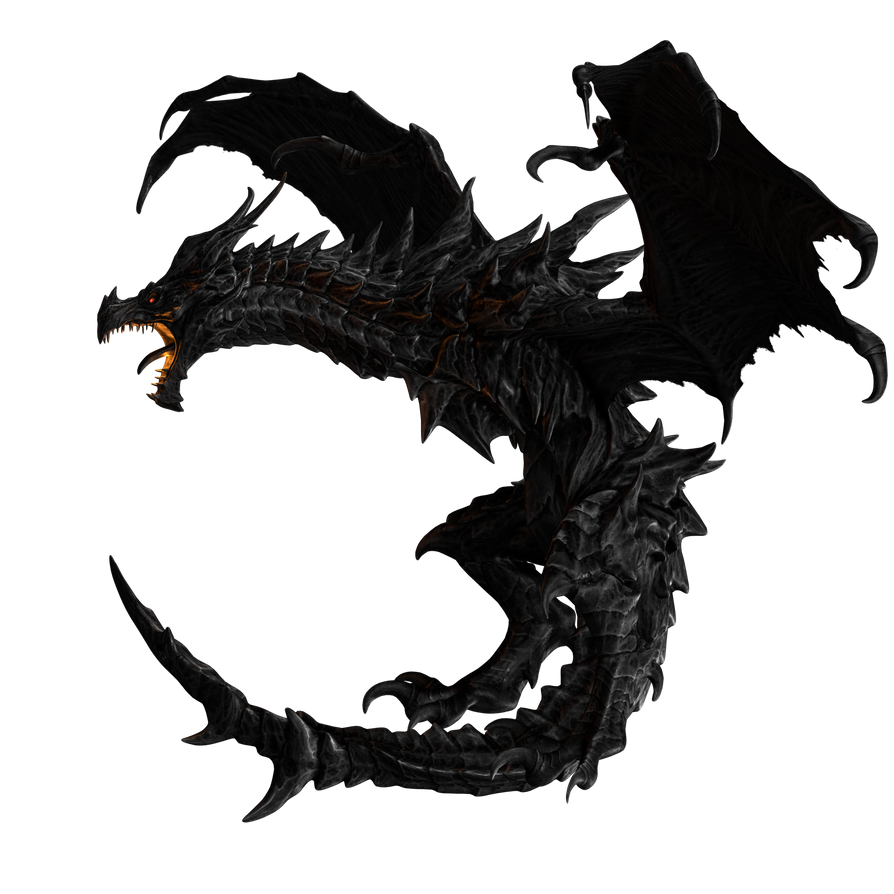
\includegraphics[width=5cm]{other/grim.png}};
    
  % Authors positioned around the outer circle
  \foreach \name/\idx in {I2 Leadership/0, Gaurang Pendharkar/1, Varun Ananth/2,
  Carter Swartout/3, Eric Ye/4, Arya Sanjay/5, Misha Nivota/6} {
    \pgfmathtruncatemacro\angle{Mod(360 / 7 * \idx + 90, 360)}
    % Calculate rotation angle for names to be always upright
    \pgfmathparse{\angle<180 ? \angle-90 : \angle+90}
    \ifnum\angle=0
    \pgfmathsetmacro\rot{\angle+90}
    \else
    \pgfmathsetmacro\rot{\pgfmathresult} % Default condition for others
    \fi

    % Author names
    \node[rotate=\rot, anchor=mid, font=\bfseries\Large] at
    (\angle:\Radius) {\name};

  }
\end{tikzpicture}\\
\texttt{v1.0} %%% VERSION NUMBER
\newpage

\begingroup
\section*{The I2 Grimoire: {{UNIT}}}
This is the {{UNIT}} unit of the I2 Grimoire book. Find the full book and other units on our website: \url{https://grimoire.uw-i2.org}.

We are Interactive Intelligence, an organization of interdisciplinary thinkers that seek to probe intelligence through the intersection of AI, neuroscience, and related fields. This book serves as a launchpad for the basic theory that underlies major AI systems and covers five large (intersecting) spheres: Machine Learning, Deep Learning, Computer Vision, Reinforcement Learning, and Language Modeling. While by no means a thorough overview of any one of these fields, this book serves as a starting point that will paint a large picture in your mind about the five aforementioned topics. This book is written in layman's english, and introduces some complex (but core) math while explaining as much intuition behind it as possible. Regardless of your background, there is something interesting you will learn in these pages. Feel free to explore sections that interest you, backtracking if you encounter unfamiliar concepts.

This book is a culmination of many months of work by very talented students from the University of Washington. It was entirely created by I2 members, and we hope that you enjoy what we have written on these pages and leave better equipped to navigate this world we share with AI algorithms.

\subsection*{Additional Information}
This book was written to pair with the Interactive Intelligence intro to NeuroAI course, which lives here: \href{https://course.uw-i2.org/}{Interactive Intelligence Intro to NeuroAI Course Website}. There are questions associated with some sections, which serve as optional exercises for you to test your understanding. If you have questions or comments on the information in this book, please contact \href{mailto:varunananth1@gmail.com}{\texttt{varunananth1@gmail.com}} \\
\vspace{1cm}
\begin{center}
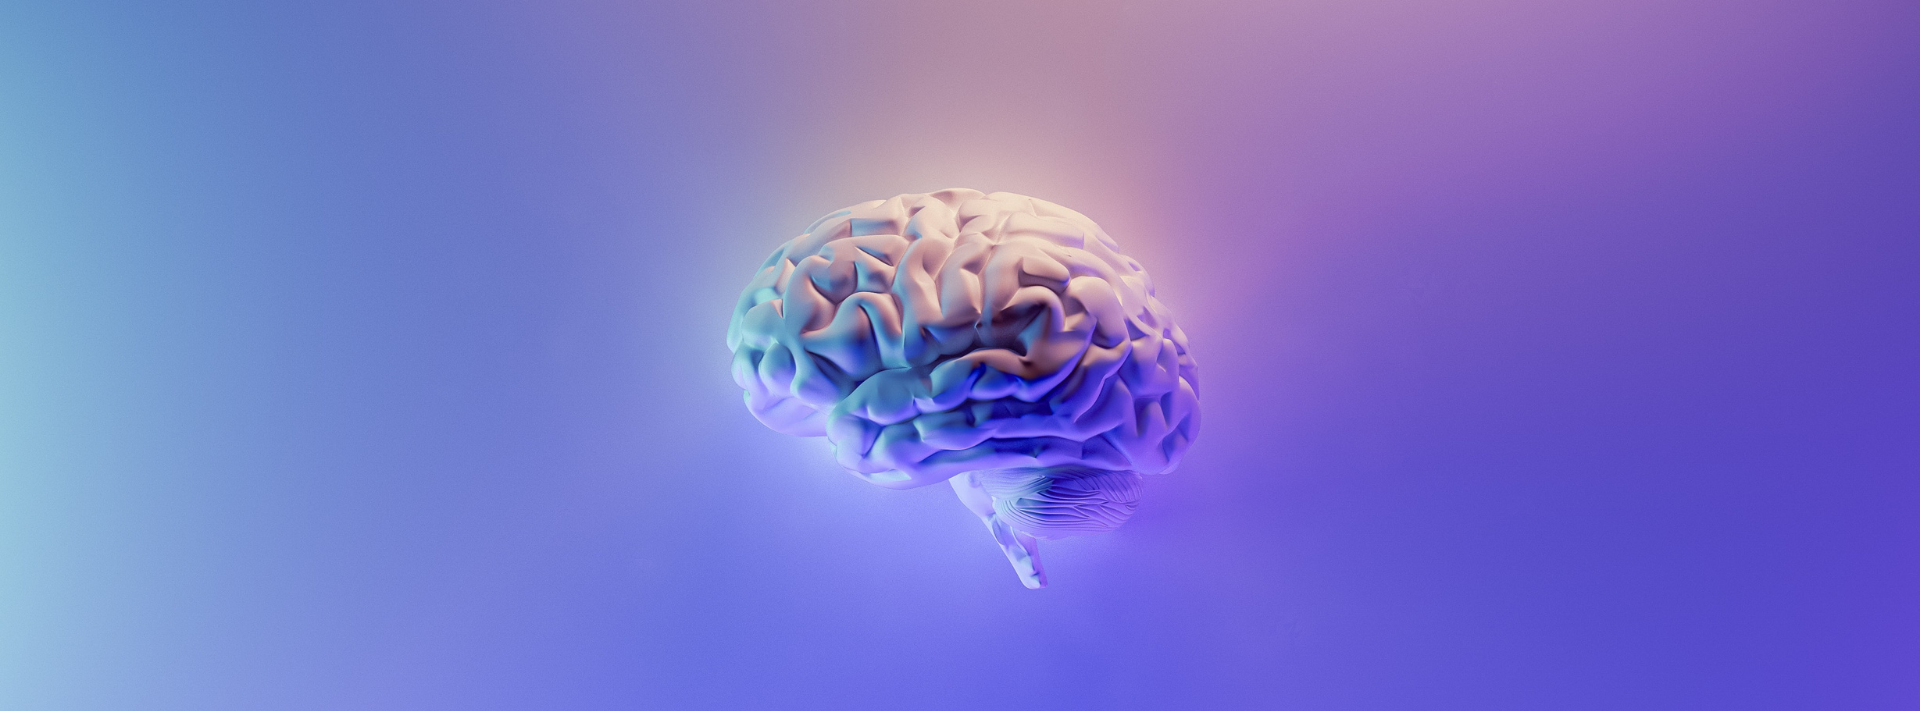
\includegraphics[scale=0.3]{other/i2-brain.png}
\end{center}
\endgroup

\newpage
\tableofcontents
\newpage

\section*{{{UNIT}}}
\include{{{unit}}}

\centering
\newpage
\begingroup
\section*{Thank You for Reading :)}
- The Interactive Intelligence Team
\endgroup

\end{document}
